\documentclass[a1paper,portrait]{tikzposter}

% Packages
\usepackage{amsmath}
\usepackage{amssymb}
\usepackage{graphicx}
\usepackage{enumitem}
\usepackage{url}
\usepackage{tikz}
\usetikzlibrary{shapes,arrows,positioning}

% Color theme - Academic
\definecolorstyle{AcademicStyle}{
    \definecolor{colorOne}{RGB}{26,54,93}      % Navy blue
    \definecolor{colorTwo}{RGB}{39,103,73}     % Forest green
    \definecolor{colorThree}{RGB}{247,250,252} % Light gray
}{
    \colorlet{backgroundcolor}{white}
    \colorlet{framecolor}{colorOne}
    \colorlet{titlefgcolor}{white}
    \colorlet{titlebgcolor}{colorOne}
    \colorlet{blocktitlebgcolor}{colorOne}
    \colorlet{blocktitlefgcolor}{white}
    \colorlet{blockbodybgcolor}{colorThree}
    \colorlet{blockbodyfgcolor}{black}
}

\usecolorstyle{AcademicStyle}
\usetitlestyle{Filled}
\useblockstyle{Minimal}

% Additional colors
\definecolor{navyblue}{RGB}{26,54,93}
\definecolor{forestgreen}{RGB}{39,103,73}
\definecolor{brickred}{RGB}{197,48,48}
\definecolor{goldaccent}{RGB}{214,158,46}
\definecolor{navybluetint}{RGB}{230,235,243}
\definecolor{forestgreentint}{RGB}{230,243,235}
\definecolor{brickredtint}{RGB}{250,230,230}
\definecolor{goldaccenttint}{RGB}{253,245,230}

\title{\textbf{Kalman Filter: A Probabilistic Approach to Signal Estimation}}
\author{Probability \& Statistics Course --- Final Project}
\institute{Interactive Demo: \url{https://leonathn.github.io/FinalProjectProbability/}}

\begin{document}

\maketitle

\begin{columns}
\column{0.33}

%==============================================================================
\block{Abstract}{
The \textbf{Kalman Filter} is an optimal recursive algorithm that estimates the state of a dynamic system from noisy measurements. This project presents an interactive web-based visualization demonstrating how the Kalman Filter applies fundamental probability concepts---including \textbf{Gaussian distributions}, \textbf{Bayes' theorem}, and \textbf{variance reduction}---to achieve superior noise filtering.

\vspace{0.5em}
\textbf{Keywords:} Kalman Filter, Bayesian Estimation, Gaussian, Variance, Signal Processing
}

%==============================================================================
\block{1. Introduction}{
In real-world applications, measurements are always corrupted by \textbf{noise}. The challenge is to estimate the \textit{true} underlying value.

\vspace{0.5em}
\textbf{Problem Statement:}
\begin{equation*}
\boxed{z_k = x_k + v_k}
\end{equation*}
where:
\begin{itemize}[leftmargin=*]
    \item $z_k$ = noisy measurement at time $k$
    \item $x_k$ = true (unknown) value
    \item $v_k \sim \mathcal{N}(0, R)$ = measurement noise
\end{itemize}

\vspace{0.5em}
\textbf{Goal:} Find the best estimate $\hat{x}_k$ that minimizes the estimation error variance.
}

%==============================================================================
\block{2. Probability Foundations}{
The Kalman Filter is built on key probability concepts:

\vspace{0.5em}
\textbf{\textcolor{forestgreen}{Gaussian (Normal) Distribution:}}
\begin{equation*}
p(x) = \frac{1}{\sqrt{2\pi\sigma^2}} \exp\left(-\frac{(x-\mu)^2}{2\sigma^2}\right)
\end{equation*}

\textbf{\textcolor{goldaccent}{Variance as Uncertainty:}}
\begin{equation*}
\text{Var}(X) = \sigma^2 = E[(X - \mu)^2]
\end{equation*}

\textbf{\textcolor{brickred}{Bayes' Theorem:}}
\begin{equation*}
P(\text{state} | \text{meas}) = \frac{P(\text{meas} | \text{state}) \cdot P(\text{state})}{P(\text{meas})}
\end{equation*}

The Kalman Filter is \textbf{recursive Bayesian estimation}!
}

%==============================================================================
\block{3. Intuitive Understanding}{
\textbf{The Kalman Gain as a ``Trust Factor'':}

\vspace{0.5em}
\begin{center}
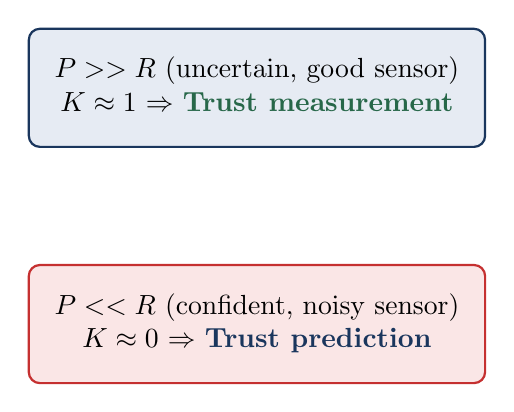
\begin{tikzpicture}[scale=1.2]
    \node[draw=navyblue, thick, fill=navybluetint, rounded corners, minimum width=5cm, minimum height=1.5cm] at (0,0) {
        \begin{tabular}{c}
        $P >> R$ (uncertain, good sensor)\\
        $K \approx 1$ $\Rightarrow$ \textcolor{forestgreen}{\textbf{Trust measurement}}
        \end{tabular}
    };
    \node[draw=brickred, thick, fill=brickredtint, rounded corners, minimum width=5cm, minimum height=1.5cm] at (0,-2.5) {
        \begin{tabular}{c}
        $P << R$ (confident, noisy sensor)\\
        $K \approx 0$ $\Rightarrow$ \textcolor{navyblue}{\textbf{Trust prediction}}
        \end{tabular}
    };
\end{tikzpicture}
\end{center}

\vspace{0.5em}
\textbf{GPS Analogy:}
\begin{itemize}[leftmargin=*]
    \item \textcolor{navyblue}{\textbf{Prediction:}} ``Based on speed, I should be HERE''
    \item \textcolor{brickred}{\textbf{Measurement:}} ``Satellite says THERE (noisy!)''
    \item \textcolor{goldaccent}{\textbf{Result:}} ``Truth is somewhere in between''
\end{itemize}
}

%==============================================================================
\column{0.34}

%==============================================================================
\block{4. The Kalman Filter Algorithm}{
The filter operates in two phases: \textbf{Predict} and \textbf{Update}.

\vspace{0.5em}
\begin{center}
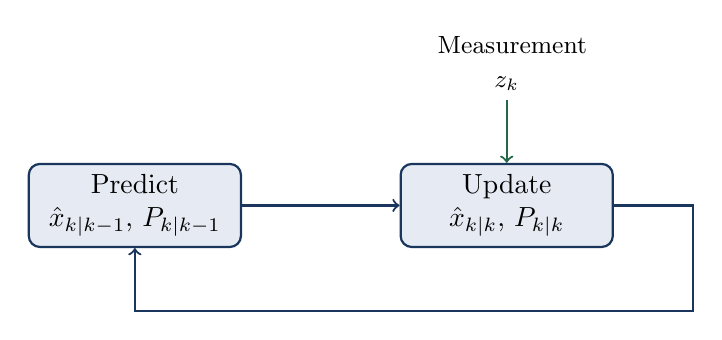
\begin{tikzpicture}[node distance=2cm, auto,
    block/.style={rectangle, draw=navyblue, thick, fill=navybluetint, text width=7em, text centered, rounded corners, minimum height=3em},
    arrow/.style={->, thick, navyblue}]
    
    \node[block] (predict) {Predict\\$\hat{x}_{k|k-1}$, $P_{k|k-1}$};
    \node[block, right=of predict] (update) {Update\\$\hat{x}_{k|k}$, $P_{k|k}$};
    \node[above=0.8cm of update, text width=5em, text centered] (meas) {\small Measurement $z_k$};
    
    \draw[arrow] (predict) -- (update);
    \draw[arrow] (update.east) -- ++(1,0) |- ([yshift=-0.8cm]predict.south) -- (predict.south);
    \draw[arrow, forestgreen] (meas) -- (update);
\end{tikzpicture}
\end{center}

\vspace{1em}
\coloredbox[bgcolor=navybluetint,framecolor=navyblue]{
\textbf{\textcolor{navyblue}{Step 1: Prediction}}
\begin{align*}
\hat{x}_{k|k-1} &= \hat{x}_{k-1|k-1}\\
P_{k|k-1} &= P_{k-1|k-1} + Q
\end{align*}
}

\vspace{0.5em}
\coloredbox[bgcolor=forestgreentint,framecolor=forestgreen]{
\textbf{\textcolor{forestgreen}{Step 2: Kalman Gain}}
\begin{equation*}
\boxed{K_k = \frac{P_{k|k-1}}{P_{k|k-1} + R}}
\end{equation*}
$K$ determines trust: measurement vs prediction
}

\vspace{0.5em}
\coloredbox[bgcolor=goldaccenttint,framecolor=goldaccent]{
\textbf{\textcolor{goldaccent}{Step 3: State Update}}
\begin{equation*}
\boxed{\hat{x}_{k|k} = \hat{x}_{k|k-1} + K_k(z_k - \hat{x}_{k|k-1})}
\end{equation*}
Weighted average toward measurement
}

\vspace{0.5em}
\coloredbox[bgcolor=brickredtint,framecolor=brickred]{
\textbf{\textcolor{brickred}{Step 4: Covariance Update}}
\begin{equation*}
\boxed{P_{k|k} = (1 - K_k) P_{k|k-1}}
\end{equation*}
Uncertainty \textbf{decreases} after measurement!
}
}

%==============================================================================
\block{5. Numerical Example}{
\textbf{Given:} $\hat{x}_{k-1} = 100$, $P_{k-1} = 4$, $z_k = 105$, $Q = 1$, $R = 10$

\vspace{0.5em}
\begin{center}
\begin{tabular}{|l|l|l|}
\hline
\textbf{Step} & \textbf{Formula} & \textbf{Result} \\
\hline
Predict & $P_{k|k-1} = 4 + 1$ & $P = 5$ \\
\hline
Gain & $K = \frac{5}{5+10}$ & $K = \textcolor{forestgreen}{\mathbf{0.333}}$ \\
\hline
Update & $100 + 0.333(105-100)$ & $\hat{x} = \textcolor{navyblue}{\mathbf{101.67}}$ \\
\hline
Covariance & $(1-0.333) \times 5$ & $P = \textcolor{brickred}{\mathbf{3.33}}$ \\
\hline
\end{tabular}
\end{center}

\vspace{0.5em}
\textbf{Result:} Uncertainty reduced from 5 to 3.33 (\textbf{33\% reduction!})
}

%==============================================================================
\column{0.33}

%==============================================================================
\block{6. Interactive Visualization}{
Our web-based demo at:

\vspace{0.3em}
\textbf{\url{https://leonathn.github.io/FinalProjectProbability/}}

\vspace{0.5em}
\textbf{Features:}
\begin{itemize}[leftmargin=*]
    \item \textbf{5 Data Sources:} Bitcoin, Temperature, Stocks, Sensor, GPS
    \item \textbf{Before/After Comparison:} Visual noise reduction
    \item \textbf{Adjustable Parameters:} R and Q sliders
    \item \textbf{Interactive Calculator:} Step-by-step computation
\end{itemize}

\vspace{0.5em}
\begin{center}
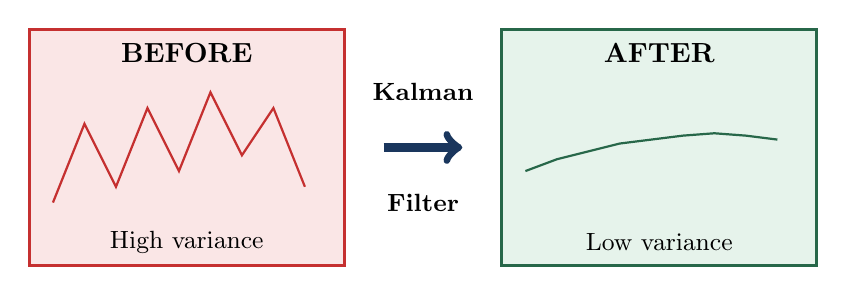
\begin{tikzpicture}[scale=1]
    % Before box
    \draw[brickred, very thick, fill=brickredtint] (0,0) rectangle (4,3);
    \node at (2,2.7) {\textbf{BEFORE}};
    \draw[brickred, thick] (0.3,0.8) -- (0.7,1.8) -- (1.1,1.0) -- (1.5,2.0) -- (1.9,1.2) -- (2.3,2.2) -- (2.7,1.4) -- (3.1,2.0) -- (3.5,1.0);
    \node at (2,0.3) {\small High variance};
    
    % Arrow
    \draw[->, line width=3pt, navyblue] (4.5,1.5) -- (5.5,1.5);
    \node at (5,2.2) {\small\textbf{Kalman}};
    \node at (5,0.8) {\small\textbf{Filter}};
    
    % After box
    \draw[forestgreen, very thick, fill=forestgreentint] (6,0) rectangle (10,3);
    \node at (8,2.7) {\textbf{AFTER}};
    \draw[forestgreen, thick] (6.3,1.2) -- (6.7,1.35) -- (7.1,1.45) -- (7.5,1.55) -- (7.9,1.6) -- (8.3,1.65) -- (8.7,1.68) -- (9.1,1.65) -- (9.5,1.6);
    \node at (8,0.3) {\small Low variance};
\end{tikzpicture}
\end{center}
}

%==============================================================================
\block{7. Results \& Validation}{
\begin{center}
\begin{tabular}{|l|c|c|}
\hline
\textbf{Metric} & \textbf{Raw} & \textbf{Filtered} \\
\hline
Variance & High & \textcolor{forestgreen}{\textbf{-40 to -70\%}} \\
\hline
Trend Preserved & -- & \textcolor{forestgreen}{\checkmark} \\
\hline
Responsiveness & -- & \textcolor{forestgreen}{\checkmark} \\
\hline
Lag/Delay & -- & \textcolor{forestgreen}{Minimal} \\
\hline
\end{tabular}
\end{center}

\vspace{0.5em}
\textbf{Key Findings:}
\begin{enumerate}[leftmargin=*]
    \item Noise reduction consistent across all data types
    \item Filter adapts via Kalman Gain
    \item Real-time performance achieved
\end{enumerate}
}

%==============================================================================
\block{8. Applications}{
\begin{itemize}[leftmargin=*]
    \item \textbf{\textcolor{navyblue}{Navigation:}} GPS, drones, spacecraft
    \item \textbf{\textcolor{forestgreen}{Finance:}} Stock prediction, trading
    \item \textbf{\textcolor{goldaccent}{Robotics:}} Sensor fusion, SLAM
    \item \textbf{\textcolor{brickred}{Medical:}} ECG/EEG processing
\end{itemize}

\vspace{0.3em}
\textit{Apollo 11 used Kalman Filter to reach the Moon!}
}

%==============================================================================
\block{9. Conclusion}{
The Kalman Filter is:
\begin{enumerate}[leftmargin=*]
    \item \textbf{Fundamentally probabilistic} --- Gaussian + Bayes
    \item \textbf{Mathematically elegant} --- only 4 equations
    \item \textbf{Practically powerful} --- proven on real data
\end{enumerate}

\vspace{0.5em}
\textbf{References:}
\begin{enumerate}[leftmargin=*, label={[\arabic*]}]
    \small
    \item Kalman (1960). \textit{J. Basic Engineering}
    \item Welch \& Bishop (2006). \textit{UNC Chapel Hill}
\end{enumerate}
}

\end{columns}

\end{document}
